%! TEX program = xelatex
%! TEX root = ../main.tex
%! TEX encoding = utf-8

%%%%%%%%%%%%%%%%%%%%%%%%%%%%%%%%%%%%%%%%%%%%%%%%%%%%%%%%%%%%%%%%%%%%%%
%
%  哈尔滨工程大学学位论文 XeLaTeX 模版 —— 正文文件 chap04.tex
%
%  版本:1.0.0
%  最后更新:
%  修改者:Leo LiWenhui lwh@hrbeu.edu.cn
%  修订者:
%  编译环境1:Ubuntu 12.04 + TeXLive 2013/2014
%  编译环境2:Windows 7/8  + TeXLive 2013/2014
%
%%%%%%%%%%%%%%%%%%%%%%%%%%%%%%%%%%%%%%%%%%%%%%%%%%%%%%%%%%%%%%%%%%%%%

\chapter{数学公式的排版}[Math Equation]
\label{chap06}

\section{公式规范}[Requirement of Equation]

论文中的公式应另起行,原则上应居中书写,与周围文字留有足够的空间区分开。
若公式前有文字(如“解”、“假定”等),文字空两格写,公式仍居中写。公式末不加标点。

公式应标注序号,并将序号置于括号内。 公式序号按章编排,如第~1~章第一个公式序号为“(1-1)”。公式的序号右端对齐。

公式较长时最好在等号“=”处转行,如难实现,则可在~$+$、$-$、$\times$、$\div$~运算符号处转行,转行时运算符号仅书写于转行式前,不重复书写。

文中引用公式时,一般用“见式~(1-1)”或“由公式~(1-1)”。

公式中用斜线表示“除”的关系时应采用括号,以免含糊不清,如~$a/(b\cos x)$。通常“乘”的关系在前,如~$a\cos x/b$而不写成~$(a/b)\cos x$。

不能用文字形式表示等式,如:$\textnormal{刚度}=\frac{{\textnormal{受力}}}{{\textnormal{受力方向的位移}}}$。

\textbf{对于数学公式的输入方法,网络上有一个比较全面权威的文档~\href{http://tug.ctan.org/cgi-bin/ctanPackageInformation.py?id=voss-mathmode}{Math mode}~请大家事先大概浏览一下。下面将对学位论文中主要用到的数学公式排版形式进行阐述。}

\section{生成~LaTeX~数学公式的两种方法}[Methods of Equation]

对于先前没有接触过~\LaTeX~的人来说,编写~\LaTeX~数学公式是一件很繁琐的事,尤其是对复杂的数学公式来说,更可以说是一件难以完成的任务。
实际上,生成~\LaTeX~数学公式有一种基于~MathType~数学公式编辑器的简便方法。

MathType~是一款功能强大的数学公式编辑器软件,能够用来在文本环境中插入~Windows OLE~图形格式的复杂数学公式,所以应用比较普遍。但此软件只有~30~天的试用期,之后若再继续使用则需要付费购买才行。网络上有很多破解版的~MathType~软件可供下载免费使用,
笔者推荐下载安装版本号在~6.5~之上的中文破解版。

在安装好~MathType~之后,若在输入窗口中编写数学公式,复制到剪贴板上的仍然是图形格式的对象。
若希望得到可插入到~\LaTeX~编辑器中的文本格式对象,则需要对~MathType~软件做一下简单的设置:在~MathType~最上排的按钮中依次选择“参数选项
$\to$转换”,在弹出的对话窗中选中“转换到其它语言(文字):”,在转换下拉框中选择“Tex~--~--~LaTeX 2.09 and later”,并将对话框最下方的两个复选框全部勾掉,点击确定,这样,再从输入窗口中复制出来的对象就是文本格式的了,就可以直接将其粘贴到~\LaTeX~
编辑器中了。按照这种方法生成的数学公式两端分别有标记\verb|\[|和标记\verb|\]|,在这两个标记之间才是真正的数学公式代码。

若希望从~MathType~输入窗口中复制出来的对象为图形格式,则只需再选中“公示对象(Windows OLE~图形)”即可。


\section{行内公式}

出现在正文一行之内的公式称为行内公式,例如~$f(x)=\int_{a}^{b}\frac{\sin{x}}{x}\mathrm{d}x$。对于非矩阵和非多行形式的行内公式,一般不会使得行距发生变化,而~word~等软件却会根据行内公式的竖直距离而自动调节行距,如图~\ref{hangju}~所示。
\begin{figure}[htbp]
  \centering
  \subfigure{\label{latex}}\addtocounter{subfigure}{-2}
  \subfigure[Inline mode equation derived from \LaTeX system]{\subfigure[由~\LaTeX~系统生成的行内公式]
    {\fbox{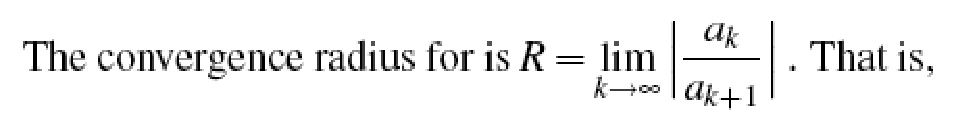
\includegraphics[width=0.55\textwidth]{latex}}}}
  \subfigure{\label{word}}\addtocounter{subfigure}{-2}
  \subfigure[Inline mode equation displayed as .doc format file derived from word software]{\subfigure[由~word软件生成的~.doc~格式行内公式]
    {\fbox{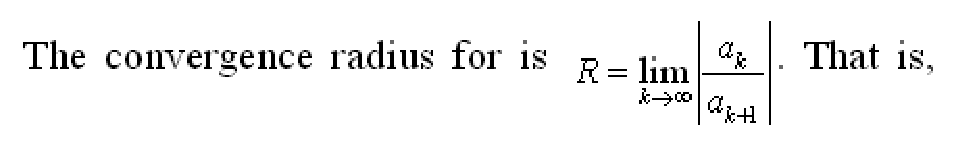
\includegraphics[width=0.55\textwidth]{word}}}}
  \subfigure{\label{pdf}}\addtocounter{subfigure}{-2}
  \subfigure[Inline mode equation displayed as .pdf format file derived from word software]{\subfigure[由~word软件生成的~.pdf~格式行内公式]
    {\fbox{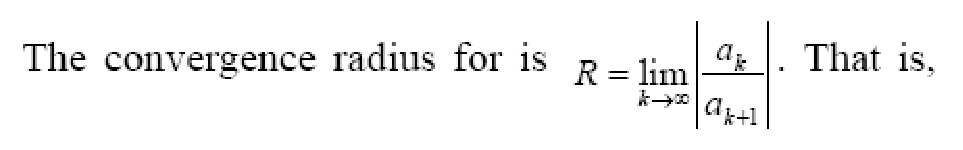
\includegraphics[width=0.55\textwidth]{pdf}}}}
  \bicaption[hangju]{}{由~\LaTeX~和~word~生成的~3~种行内公式屏显效果}{Fig.$\!$}{Three kinds of inline mode equation displayed effects derived from \LaTeX and word}
  \vspace{-1em}
\end{figure}
这三幅图分别为~\LaTeX~和~word~生成的行内公式屏显效果,从图中可看出,在~\LaTeX~文本含有公式的行内,在正文与公式之间对接工整,行距不变;而在~word~文本含有公式的行内,在正文与公式之间对接不齐,行距变大。因此从这一点来说,
\LaTeX~系统在数学公式的排版上具有很大优势。

\LaTeX~提供的行内公式最简单、最有效的方法是采用~\TeX~本来的标记——开始和结束标记都写作~\$,例如本节开始的例子可由下面的输入得到。
\begin{lstlisting}
  $f(x)=\int_{a}^{b}\frac{\sin{x}}{x}\mathrm{d}x$
\end{lstlisting}

\section{行间公式}

位于两行之间的公式称为行间公式,每个公式都是一个单独的段落,例如
\[\int_a^b{f\left(x\right)\mathrm{d}x}=\lim_{\left\|\Delta{x_i}\right\|\to 0}\sum_i{f\left(\xi_i\right)\Delta{x_i}}\]

除人工编号外,\LaTeX~各种类型行间公式的标记见表~\ref{eqtag}。
\begin{table}[htbp]
  \bicaption[eqtag]{}{各种类型行间公式的标记}{Table$\!$}{Tags for several kinds of displaymath mode equations}
  \vspace{0.5em}\centering\wuhao
  \begin{tabularx}{0.9\textwidth}{cXX}
    \toprule
             & 无编号                                                                                                             & 自动编号                                                               \\\midrule
    单行公式 & \textbackslash begin\{displaymath\}...... \textbackslash end\{displaymath\}~或~\textbackslash [...\textbackslash ] & \textbackslash begin\{equation\} ...... \textbackslash end\{equation\} \\
    多行公式 & \textbackslash begin\{eqnarray*\} ...... \textbackslash end\{eqnarray*\}                                           & \textbackslash begin\{eqnarray\} ...... \textbackslash end\{eqnarray\} \\
    \bottomrule
  \end{tabularx}
\end{table}

另外,在自动编号的某行公式行尾添加标签~\verb|\nonumber|,可将该行转换为无编号形式。

行间多行公式需采用~\verb|eqnarray|~或~\verb|eqnarray*|~环境,它默认是一个列格式为~\verb|rcl|~的~3~列矩阵,并且中间列的字号要小一些,因此通常只将需要对齐的运算符号(通常为等号“=”)置于中间列。

对于不需要进行公示编号的行间公式,也可以使用简化的行间公式符号~\verb|$$  $$|~或~\verb|\[  \]|~,例如:

$$(\sum_{k=\frac12}^{N^2})$$
或
\[(\sum_{k=\frac12}^{N^2})\]

上述量化公式代码分别为:
\begin{lstlisting}
   $$(\sum_{k=\frac12}^{N^2})$$
 \end{lstlisting}
和
\begin{lstlisting}
   \[(\sum_{k=\frac12}^{N^2})\]
 \end{lstlisting}

\section{可自动调整大小的定界符}[Limiter Setting]

若在左右两个定界符之前分别添加命令~\verb|\left|~和~\verb|\right|,则定界符可根据所包围公式大小自动调整其尺寸,这可从式(\ref{nodelimiter})和式(\ref{delimiter})中看出。
\begin{equation}\label{nodelimiter}
  (\sum_{k=\frac12}^{N^2})
\end{equation}
\begin{equation}\label{delimiter}
  \left(\sum_{k=\frac12}^{N^2}\right)
\end{equation}
式(\ref{nodelimiter})和式(\ref{delimiter})是在~\LaTeX~中分别输入如下代码得到的。
\begin{lstlisting}
  \begin{equation}\label{nodelimiter}
    (\sum_{k=\frac12}^{N^2})
  \end{equation}
  \begin{equation}\label{delimiter}
    \left(\sum_{k=\frac12}^{N^2}\right)
  \end{equation}
\end{lstlisting}

\verb|\left|~和~\verb|\right|~总是成对出现的,若只需在公式一侧有可自动调整大小的定界符,则只要用“.”代替另一侧那个无需打印出来的定界符即可。

若想获得关于此部分内容的更多信息,可参见~\href{http://tug.ctan.org/cgi-bin/ctanPackageInformation.py?id=voss-mathmode}{Math mode}~文档的第~8~章“Brackets, braces and parentheses”。

\section{数学重音符号}[Math Symbols]

数学重音符号通常用来区分同一字母表示的不同变量,输入方法如下(需要调用~\verb|amsmath|~宏包):

{\vspace{0.5em}\noindent\wuhao\begin{tabularx}{\textwidth}{Xc|Xc|Xc}
  \verb|\acute| & $\acute{a}$ & \verb|\mathring|           & $\mathring{a}$           & \verb|\underbrace|          & $\underbrace{a}$          \\
  \verb|\bar|   & $\bar{a}$   & \verb|\overbrace|          & $\overbrace{a}$          & \verb|\underleftarrow|      & $\underleftarrow{a}$      \\
  \verb|\breve| & $\breve{a}$ & \verb|\overleftarrow|      & $\overleftarrow{a}$      & \verb|\underleftrightarrow| & $\underleftrightarrow{a}$ \\
  \verb|\check| & $\check{a}$ & \verb|\overleftrightarrow| & $\overleftrightarrow{a}$ & \verb|\underline|           & $\underline{a}$           \\
  \verb|\dddot| & $\dddot{a}$ & \verb|\overline|           & $\overline{a}$           & \verb|\underrightarrow|     & $\underrightarrow{a}$     \\
  \verb|\ddot|  & $\ddot{a}$  & \verb|\overrightarrow|     & $\overrightarrow{a}$     & \verb|\vec|                 & $\vec{a}$                 \\
  \verb|\dot|   & $\dot{a}$   & \verb|\tilde|              & $\tilde{a}$              & \verb|\widehat|             & $\widehat{a}$             \\
  \verb|\grave| & $\grave{a}$ & \verb|\underbar|           & $\underbar{a}$           & \verb|\widetilde|           & $\widetilde{a}$           \\
  \verb|\hat|   & $\hat{a}$
\end{tabularx}\vspace{0.5em}}

当需要在字母~$i$~和~$j$~的上方添加重音符号时,为了去掉这两个字母顶上的小点,这两个字母应该分别改用~\verb|\imath|~和~\verb|\jmath|。

如果遇到某些符号不知道该采用什么命令能输出它时,则可通过~\href{http://detexify.kirelabs.org/classify.html}{Detexify$^2$~网站}来获取符号命令。若用鼠标左键在此网页的方框区域内画出你所要找的符号形状,则会在网页右方列出和你所画符号形状相近的~5~个符号及其相对应的~\LaTeX~输入命令。若所列出的符号中不包括你所要找的符号,还可通过点击“Select from the complete list!”的链接以得分从低到高的顺序列出所有符号及其相对应的~\LaTeX~输入命令。

最后,建议大家还是要以~\href{http://tug.ctan.org/cgi-bin/ctanPackageInformation.py?id=voss-mathmode}{Math mode}~这篇~pdf~文档作为主要参考。若要获得最为标准、美观的数学公式排版形式,可以查查文档中是否有和你所要的排版形式相同或相近的代码段,通过修改代码段以获得你所要的数学公式排版形式。

\section{定理和定义等}[Theorem]
\begin{theorem}[\cite{cnproceed}]
  宇宙大爆炸是一种爆炸。
\end{theorem}
\begin{definition}[(霍金)]
  宇宙大爆炸是一种爆炸。
\end{definition}
\begin{assumption}
  宇宙大爆炸是一种爆炸。
\end{assumption}
\begin{lemma}
  宇宙大爆炸是一种爆炸。
\end{lemma}
\begin{corollary}
  宇宙大爆炸是一种爆炸。
\end{corollary}
\begin{exercise}
  宇宙大爆炸是一种爆炸。
\end{exercise}
\begin{problem}[(Albert Einstein)]
宇宙大爆炸是一种爆炸。
\end{problem}
\begin{remark}
  宇宙大爆炸是一种爆炸。
\end{remark}
\begin{axiom}[(爱因斯坦)]
  宇宙大爆炸是一种爆炸。
\end{axiom}
\begin{conjecture}
  宇宙大爆炸是一种爆炸。
\end{conjecture}

\section{数学公式排版示例}[Equation Demo]

下面是采用~\LaTeX~实现的几个简单的数学公式排版。

这是两个采用行内格式的数学公式,行内数学公式不带编号:

$f(x) = 3x + 7$

下面是几个采用行间格式排版的数学公式,行间数学公式在最右侧自动编号,在两个~\verb|$|~符号中间进行定义:

\begin{definition}
  任给集合~$X \in U$ 和属性集~$R$, 对~$0\leqslant l < u \leqslant 1$,
  集合~$X$ 的~$l${--}下近似、$u${--}上近似分别定义为
  \begin{align}
    \underline {R} _u (X) & =  \bigcup \left\{ {X_i  \in U/R\Bigm|X_i \mathop  \subseteq \limits^u  X} \right\}, \\
    \overline {R} _l (X)  & =  \bigcup \left\{ {X_i  \in U/R\Bigm|X_i \mathop  \subset \limits^l X} \right\}.
  \end{align}
\end{definition}

\begin{theorem}[\heiti 费马]
  {\upshape\kaishu 不存在使得~
    \begin{equation}
      x^n+y^n=z^n
    \end{equation}
    成立的整数~$x$, $y$, $z$ and $n>2$. }
\end{theorem}

\begin{proof}
  {\upshape\kaishu 这是推论
    \begin{equation}
      \textcolor[rgb]{0.00,0.00,1.00}{
      I'_{{\rm{total}}} = \sum\limits_{i = 1}^n
      {\left( {M_0 V_i - M_{i{\rm{rp}}} \sqrt{V_i^2 - V_{50}^2}}\right)}}
    \end{equation}}
\end{proof}

下面是一个稍微一些复杂的公式:

\begin{equation}
  {\mu _X}\sigma _X^2\sum\limits_{i = 1}^n {{{({X_i} - \bar X)}^2}} \frac{{x - \mu }}{\sigma }\frac{{{\partial ^2}\Omega }}{{\partial u\partial v}}\oiiint\nolimits_{x \in }
  {\bigcup\limits_{i = 1}^n {{X_i}} \frac{{dy}}{{dx}}}
\end{equation}

利用~\LaTeX~你可以排出专业的数学版面效果。


\section*{本章小结}[Brief Summary]
数学公式排版方法介绍。
